\FloatBarrier

\begin{figure}[h!]
	\centering
	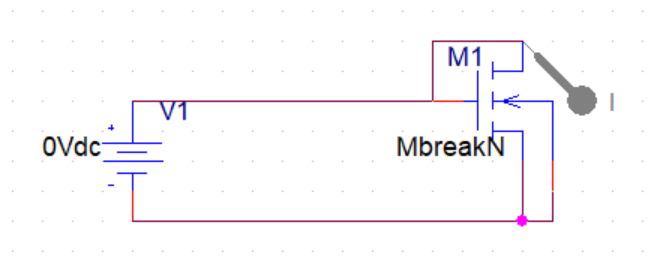
\includegraphics[scale=0.75]{./images/circuit3.PNG}
	\caption{Diode-Connected NMOS Circuit}
	\label{fig:circuit3}
\end{figure}

\FloatBarrier

Two operation modes are possible for the circuit in figure (\ref{fig:circuit3}). In the first case, consider $V_{GS} < V_{T}$. At this point, the transistor is in cutoff mode, and no current flows. For the second case, $V_{GS} > V_{T}$. Since $V_{G} = V_{D}$ and $V_{GS} > V_{GS} - V_{T}$, $V_{DS} > V_{GS} - V_{T}$. This satisfies the condition for saturation. So, the transistor is either in cutoff or in saturation. So, the transistor's drain current is given by: \\

\begin{equation}
	\label{eq:diode_drain_current}
	i_{D} =
	\begin{cases}
		\frac{k_n}{2} ( V_{GS} - V_{T} )^2 & V_{GS} > V_{T} \\
		0 & V_{GS} < V_{T}
	\end{cases}
\end{equation}

This current behavior mimics that of a pn-junction diode, but with a current that varies quadratically instead of exponentially with the applied voltage $V_{GS}$. The transistor, like a diode, requires a certain voltage in order to "turn-on", specifically $V_{T}$. Once this voltage is exceeded, the transistor is activated and immediately enters the saturation region. From this, increasing $V_{GS}$ leads to quadratically larger drain currents, just like how increasing the applied voltage leads to exponentially growing diode currents.

\FloatBarrier

\begin{figure}[h!]
	\centering
	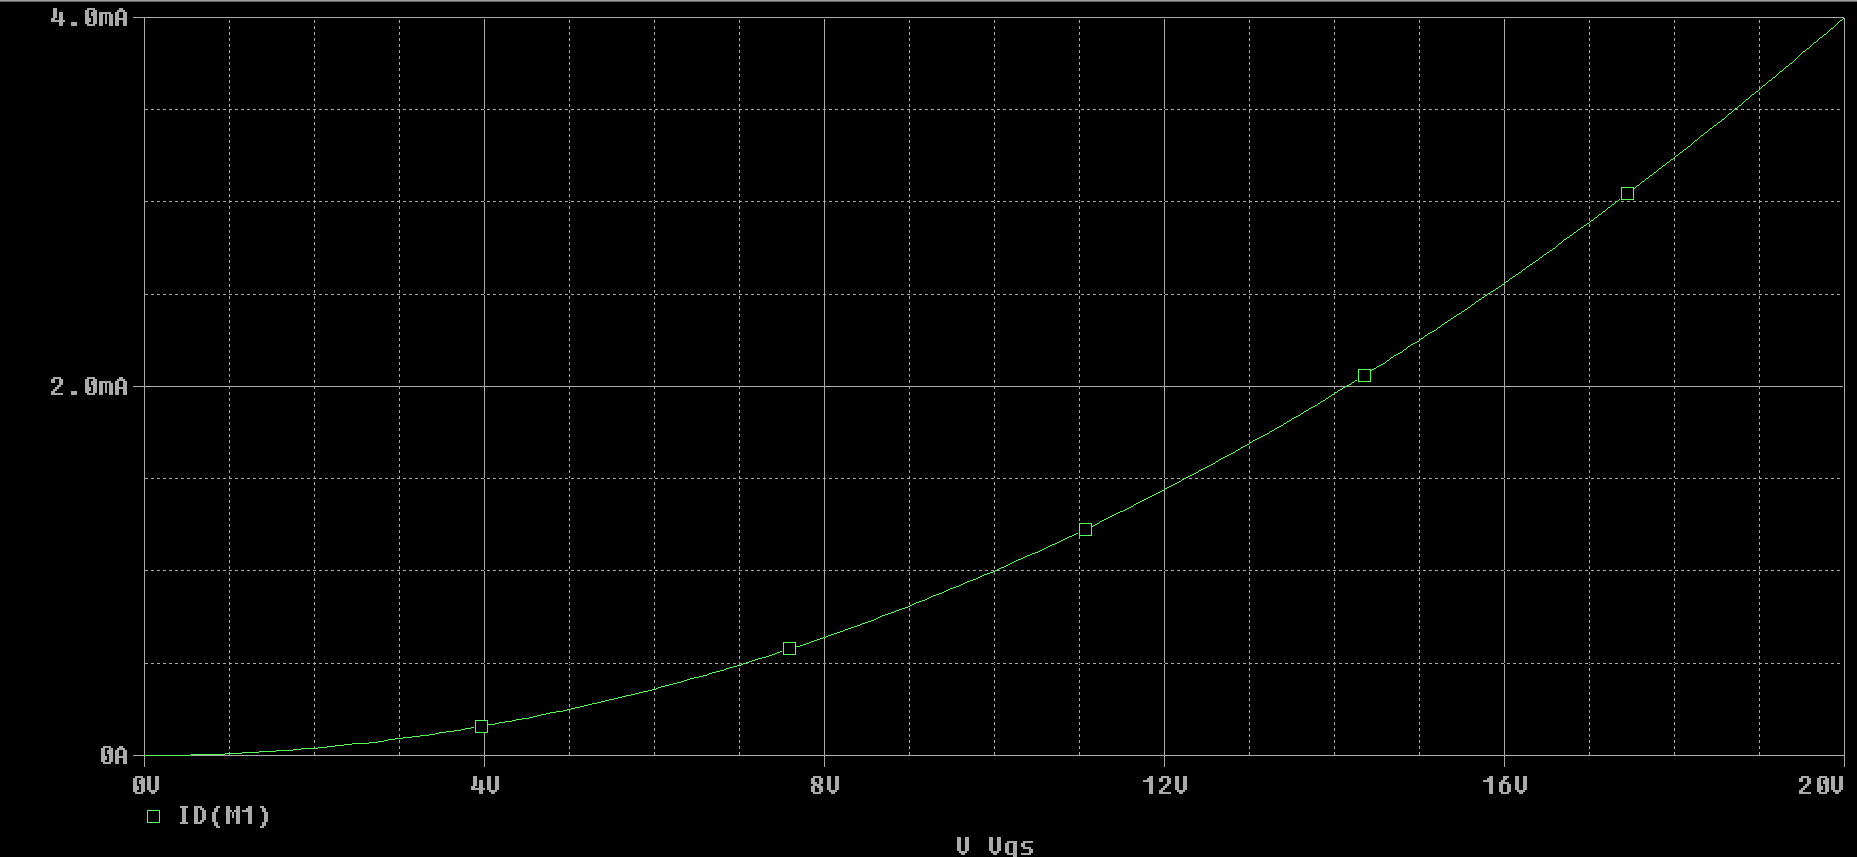
\includegraphics[scale=0.50]{./images/circuit3_dc_sweep.PNG}
	\caption{DC Sweep of Circuit in Figure (\ref{fig:circuit3})}
	\label{fig:circuit3_dc_sweep}
\end{figure}

\FloatBarrier
